\documentclass[30pt,twocolumn,letterpaper]{article}
\usepackage{cvpr}
\usepackage{times}
\usepackage{booktabs}
\usepackage{epsfig}
\usepackage{graphicx}
\usepackage{amsmath}
\usepackage{amssymb}
\cvprfinalcopy
\def\cvprPaperID{****}
\def\httilde{\mbox{\tt\raisebox{-.5ex}{\symbol{126}}}}
\usepackage{graphicx}
\usepackage{indentfirst}
\setlength{\parindent}{2em}
\usepackage{cite}
\usepackage[colorlinks,linkcolor=red,anchorcolor=blue,citecolor=green,backref=page]{hyperref}
\author{Qilei Zhang\\\\
Jul 14 2018}
\title{Reliable Logic Circuit Elements that Exploit Nonlinearity in the Presence of a Noise Floor}
\begin{document}
\maketitle
\begin{abstract}
  The response of noisy nonlinear systems to deterministic input signals can be enhanced by cooperative phenomena. When a two square wave is used as input to the two state, the response of the system can produce the logical output of the probability controlled by the noise intensity (NOR = OR). When a noise is added (for fixed threshold or nonlinearity), the probability of reflecting the output of NOR = or operation increases to a unit and then decreases.
\end{abstract}
\section{Introduction}
Over the last few years, it has become increasingly obvious that understanding how noise and nonlinearity cooperate, in a dynamical system, to produce novel effects is critical in understanding how complex systems behave and evolve\cite{Choudhury1977Reliability}. \\

\par
Stochastic resonance provides one such example wherein the cooperative behavior between noise and dynamics produces interesting, often counterintuitive, physical phenomena. SR has received much attention over the past few decades and consists of the enhancement of weak input signals through a delicate interplay between the signal, noise, and nonlinearity\cite{Dokouzgiannis1987A}.
\begin{figure}[htbp]
\small
\centering
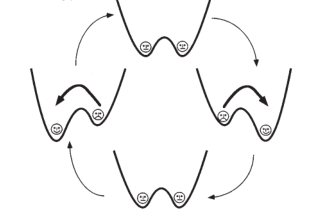
\includegraphics[width=20em]{000.png}
\caption{Each panel has
2 curves. Solid curves represent the solution x(t) from numerical
simulations for additive noise intensities D equal to (top to
bottom) 0.01, 0.5, and 1. The input I is the sum of randomly
switched square pulse trains (see text), and is the same (dashed
line) in each panel. For an optimal noise intensity (center panel)
a reliable OR=NOR gate is obtained.
}
\label{fig:lable}
\end{figure}\\
\section{Content}
As computing equipment and platform size shrink and speed increase, we are faced with more and more basic noise characteristics which cannot be suppressed or eliminated. Therefore, the understanding of the cooperative behavior between the base and the nonlinearity of the equipment noise will play a more and more important role in the design and development of the future computing concepts and equipment\cite{Murali2009Realization}.\\
\begin{table}
\begin{center}
\begin{tabular}{ccccc}
\toprule
 Input Set (I1, I2)& OR  &AND&NOR&NAND\\
\midrule
(0,0)&0&0   &1  &1\\
(0,1)/(1,0)&1  &0  &0   &1\\
(1,1)   &1  &1    &0    &0\\
 \bottomrule
\end{tabular}
\end{center}
\caption{NOR (or the NAND) gates logic operations}
\end{table}
\par
The article shows how to use the interaction between noise base and nonlinearity to design the key logic gates. In particular, the direct and flexible implementation of the basic logic gates NOR and NAND in an optimal noise band has been demonstrated, and any general computing device can be built. In addition, we demonstrate the use of nonlinearity as a logical response controller to switch logic functions\cite{Murali2009Reliable}.\\
{\small
\bibliographystyle{ieee}
\bibliography{1}
}
\end{document}
